% Part 2:
%  - Protocols
%  - Seeder/leecher
%  - Software
%  - eMule, Limewire, Bittorrent, Freenet, Kazaa, Napster
%  - Security
%  - Trackers
%  - P2P file sharing free : Skype
%  - CDN/DNS

% Sources
% howstuffWorks.com
% Cours NetArch de Fourmaux
% http://www.slideshare.net/uschmidt/peertopeer-systems
% http://en.wikipedia.org/wiki/Peer-to-peer

% 
\section{How it works?}

  \begin{frame}
    \tableofcontents[currentsection, hideothersubsections]
  \end{frame}

  \subsection{Technical challenges of P2P}
    \begin{frame}
      \frametitle{\secname}
      \framesubtitle{\subsecname}
      \begin{itemize}
        \item How Peers know each other?
        \item How to find the required file in the network?
        \item How to be sure all peers participate ?
        \item How to guarantee file availability? (seeding)
      \end{itemize}
    \end{frame}

  \subsection{Napster the grandpa}
    \begin{frame}
      \frametitle{\secname}
      \framesubtitle{\subsecname}
      \begin{itemize}
        \item Based on central index server 
        \item Server know all peers
        \item P2P only for file transfert
        \item Still some client/server !
        \item No mecasim to promote seeding
      \end{itemize}
      \begin{figure}
        \centering
        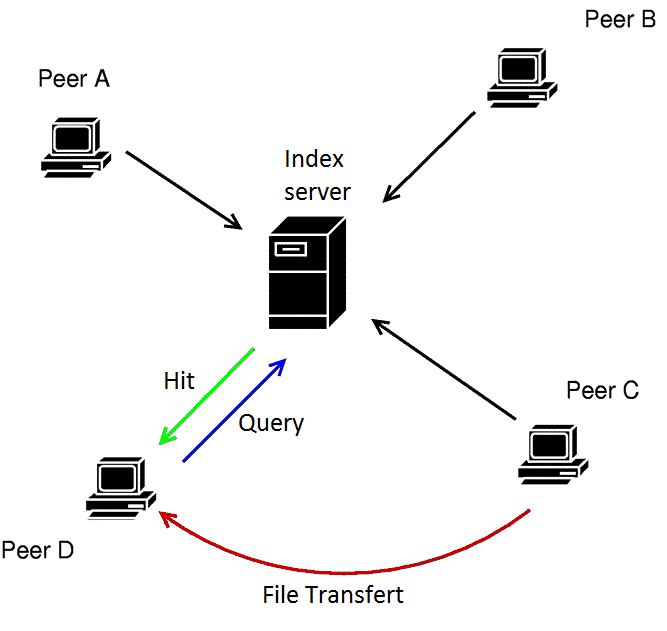
\includegraphics[scale=0.2]{img/P2-napsterProtocol2_colored.png}
        %\caption{Napster architecture}
      \end{figure}
    \end{frame}


  \subsection{Gnutella the unknown child}
    \begin{frame}
      \frametitle{\secname}
      \framesubtitle{\subsecname}
      \begin{itemize}
        \item Fully distibuted
        \item A peer know a few amount of his fellow
        \item Search by flooding
        \item Still no mechanism to promote seeding
      \end{itemize}
      \begin{figure}
        \centering
        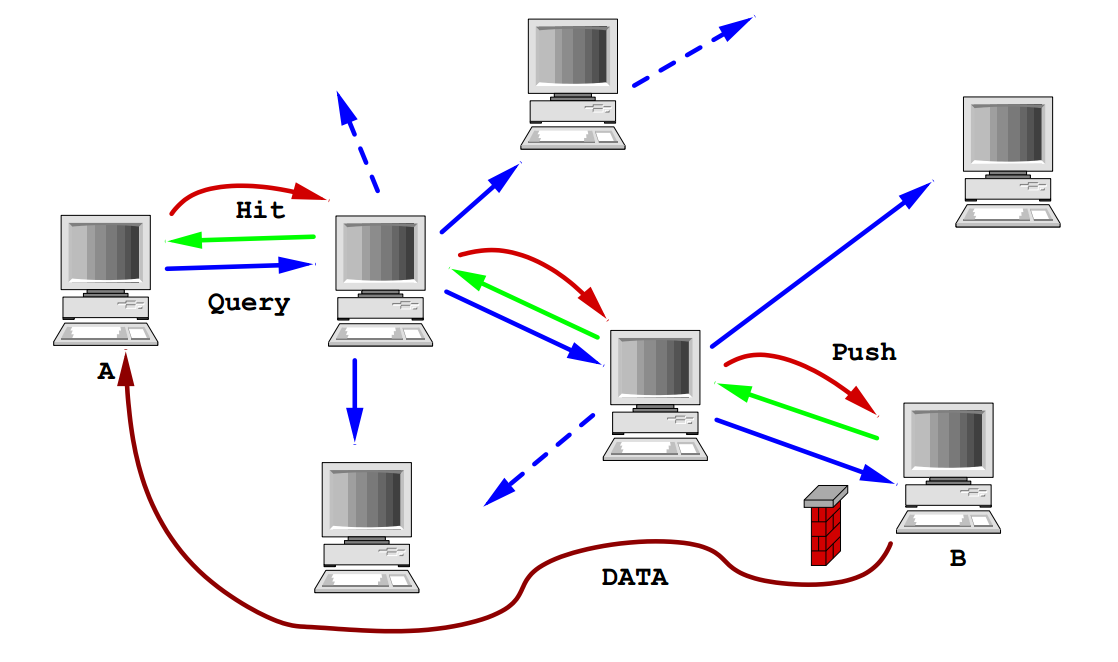
\includegraphics[scale=0.30]{img/P2-gnutellaProtocol.png}
      \end{figure}
    \end{frame}
    
    
  \subsection{Bittorent the long-living}
    \begin{frame}
      \frametitle{\secname}
      \framesubtitle{\subsecname}
      \begin{itemize}
        \item File search outsourced with .torent file
        \item A Tracker oversees the distribution
        \item Files are divided in chunk
        \item tit-for-tat policy
      \end{itemize}
    \end{frame}
   

  \subsection{Other P2P systems}
    \begin{frame}
      \frametitle{\secname}
      \framesubtitle{\subsecname}
      \begin{itemize}
        \item Internet routing
        \item IM, VoIP (SIP Protocol, Skype)
        \item CDN and others cloud based applications
        \item Grid computing, DNS
      \end{itemize}
    \end{frame}
